\begin{figure}[H]
\centering
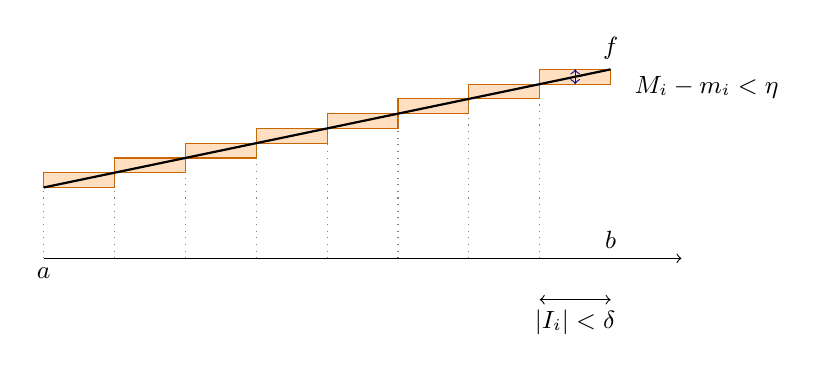
\begin{tikzpicture}[x=1.8cm,y=1.5cm,font=\small]
\foreach \i in {0,...,7}{
\pgfmathsetmacro{\a}{.5*\i}
\pgfmathsetmacro{\b}{\a+.5}
\pgfmathsetmacro{\lo}{.6+.25*\a}
\pgfmathsetmacro{\hi}{.6+.25*\b}
\filldraw[fill=orange!25,draw=orange!80!black] (\a,\lo) rectangle (\b,\hi);
\draw[gray,dotted] (\a,0)--(\a,\lo);
}
\draw[->] (0,0)--(4.5,0);
\draw[thick] (0,.6)--(4,1.6) node[above] {$f$};
\draw[<->,blue!65!black] (3.75,1.475)--(3.75,1.6);
\node[right] at (4.1,1.45) {$M_i-m_i<\eta$};
\draw[<->] (3.5,-.35)--(4,-.35) node[midway,below] {$|I_i|<\delta$};
\node[below] at (0,0) {$a$};\node[above] at (4,0) {$b$};
\end{tikzpicture}
\caption{Uniform continuity makes the vertical oscillation bands narrow
on every sufficiently short cell. Their total area is at most the common
height bound times the full interval length. The strict cell bound shown
here holds for continuous functions since extrema are attained; the proof
needs only the weak bound.}
\label{fig:uniform-bands}
\end{figure}
